\section*{Questões}
\paragraph{1.}

\begin{verbatim}
[root@localhost etc]# host -t mx dept.lr-g11.pt
dept.lr-g11.pt mail is handled by 10 mail.lr-g11.pt.
\end{verbatim}


\paragraph{2.}
Explique o que se passou. (texRes)

\begin{figure}[h]
\centering
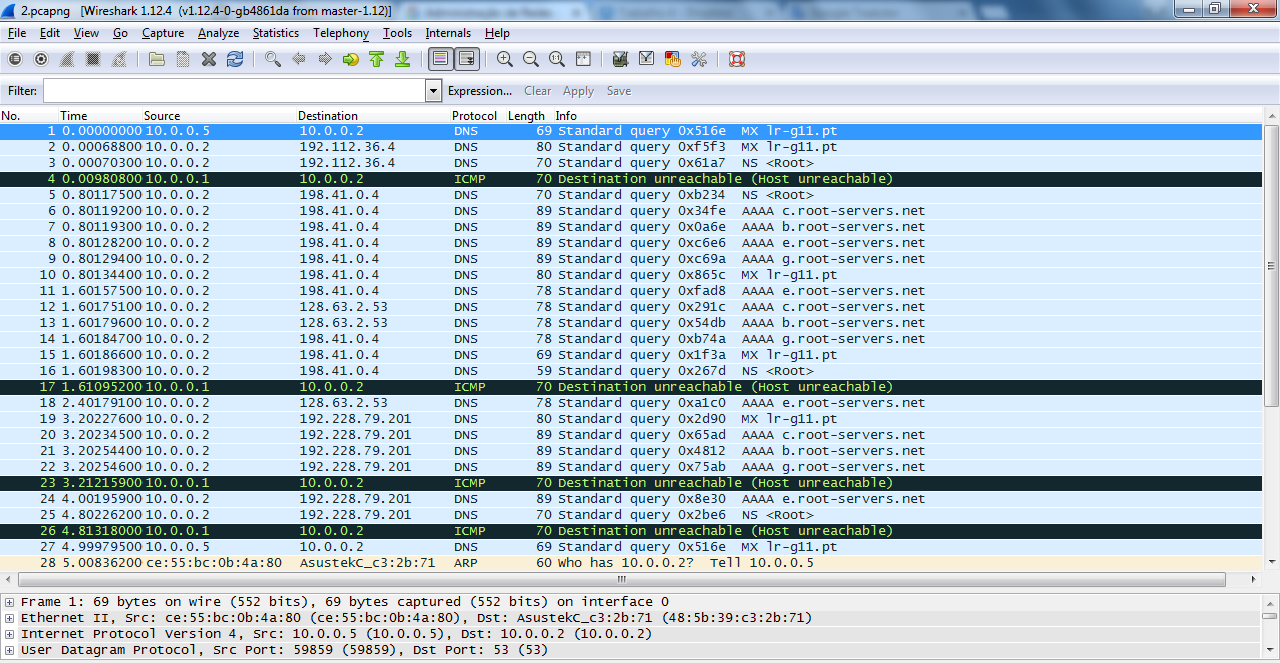
\includegraphics[width=1\textwidth, height=0.35\textheight]{2_cap.png}
\label{fig:2-capturaWireshark}
\caption{Captura \emph{wireshark} no \textsf{dns.dept.lr-gX.pt}.}
\end{figure}


%\paragraph{3.}

%\subparagraph{a.}


%\subparagraph{b.}


%\subparagraph{c.}


%\subparagraph{d.}


\paragraph{4.}
Diga o que entende por glue record e qual a sua utilidade. Foi necessário usar um nesta montagem? Em caso afirmativo, em que máquina? (texRes)


\paragraph{5.}

\subparagraph{a.}
No ficheiro \textsf{named.conf}, como podemos ver abaixo, na cláusula \textsf{options} alteramos a declaração \textsf{recursion} para \textsf{no}, e configuramos duas vistas, uma para rede interna e outra para o exterior.

\begin{verbatim}
options {
     ...
     recursion no;
     ...
};

view "interior" {
     match-clients {localhost; localnets; 172.16.0.0/24; 10.0.0.0/24;};
     recursion yes;
     zone "lr-g11.pt" IN {
     	  type master;
	  file "master/dns.lr-g11.pt.zone";
	     };
     zone "0.16.172.in-addr.arpa" IN {
        type master;
     	file "reverse/172.16.0.zone";
     };
     zone "." IN {
	type hint;
	file "named.ca";
     };
};

view "exterior" {
     match-clients {"any";};
     recursion no;
     zone "lr-g11.pt" IN {
     	  type master;
	  file "master/dns.lr-g11.pt.exterior.zone";
     };
     zone "80.168.192.in-addr.arpa" IN {
        type master;
     	file "reverse/192.168.80.zone";
     };
     zone "." IN {
	type hint;
	file "named.ca";
     };
};
\end{verbatim}

Também configuramos os ficheiros de zona para resolução direta:

\begin{verbatim}
$ORIGIN	lr-g11.pt.
$TTL	86400
@	1D	SOA dns.lr-g11.pt.	miguelferreira108.google.com. (
	2016051904
	3h
	15
	1w
	3h
	)

	NS dns.lr-g11.pt.
	MX 10 mail.lr-g11.pt.


dept NS dns.dept
dns.dept A 10.0.0.2

dns A 192.168.80.2
mail A 192.168.80.7
router A 192.168.80.1

www.lr-g11.pt CNAME dns.lr-g11.pt.
\end{verbatim}

e zona para resolução inversa:

\begin{verbatim}
$ORIGIN	80.168.192.in-addr.arpa.
$TTL	86400
@	1D	SOA dns.lr-g11.pt.	miguelferreira108.google.com. (
	2016051902
	3h
	15
	1w
	3h
	)

	NS dns.lr-g11.pt.
	MX 10 mail.lr-g11.pt.

1 PTR router.lr-g11.pt.
2 PTR dns.lr-g11.pt.
7 PTR mail.lr-g11.pt.
\end{verbatim}


\subparagraph{b.}

\begin{verbatim}
[root@localhost named]# host router.lr-g11.pt
router.lr-g11.pt has address 172.16.0.1
\end{verbatim}


\subparagraph{c.}

\begin{verbatim}
[root@localhost network-scripts]# host router.lr-g11.pt. 192.168.80.2
Using domain server:
Name: 192.168.80.2
Address: 192.168.80.2#53
Aliases: 

router.lr-g11.pt has address 192.168.80.1
\end{verbatim}


\paragraph{6.}

\subparagraph{a.}
No ficheiro \textsf{named.conf}, como podemos ver abaixo, acrescentamos as seguintes zonas:

\begin{verbatim}
zone "dept.lr-g11.pt" IN {
     type slave;
     masters {10.0.0.2;};
     file "slave/dns.dept.lr-g11.pt.zone";
};

zone "0.0.10.in-addr.arpa" IN {
     type slave;
     masters {10.0.0.2;};
     file "slave/10.0.0.zone";
};
\end{verbatim}

E também configuramos os ficheiros de zona para resolução direta:

\begin{verbatim}
$ORIGIN	dept.lr-g11.pt.
$TTL	86400
@	1D	SOA dns.dept.lr-g11.pt.	miguelferreira108.google.com. (
	2016051905
	3h
	15
	1w
	3h
	)

	NS dns.dept.lr-g11.pt.
	MX 10 mail.lr-g11.pt.


dept NS dns.dept
dns.dept A 10.0.0.2

dns A 172.16.0.2
mail A 172.16.0.7
router A 172.16.0.1

www.lr-g11.pt CNAME dns.lr-g11.pt.
\end{verbatim}

e zona para resolução inversa:

\begin{verbatim}
$ORIGIN	0.0.10.in-addr.arpa.
$TTL	86400
@	1D	SOA dns.dept.lr-g11.pt.	miguelferreira108.google.com. (
	2016051900
	3h
	15
	1w
	3h
	)

	NS dns.dept.lr-g11.pt.
	MX 10 mail.lr-g11.pt.

1 PTR router.dept.lr-g11.pt.
2 PTR dns.dept.lr-g11.pt.
7 PTR mail.lr-g11.pt.
\end{verbatim}

\newpage
\subparagraph{b.}
Captura da transferência do domínio \textsf{dept.lr-gX.pt} do \textsf{master} para o \textsf{slave}:

\begin{figure}[h]
\centering
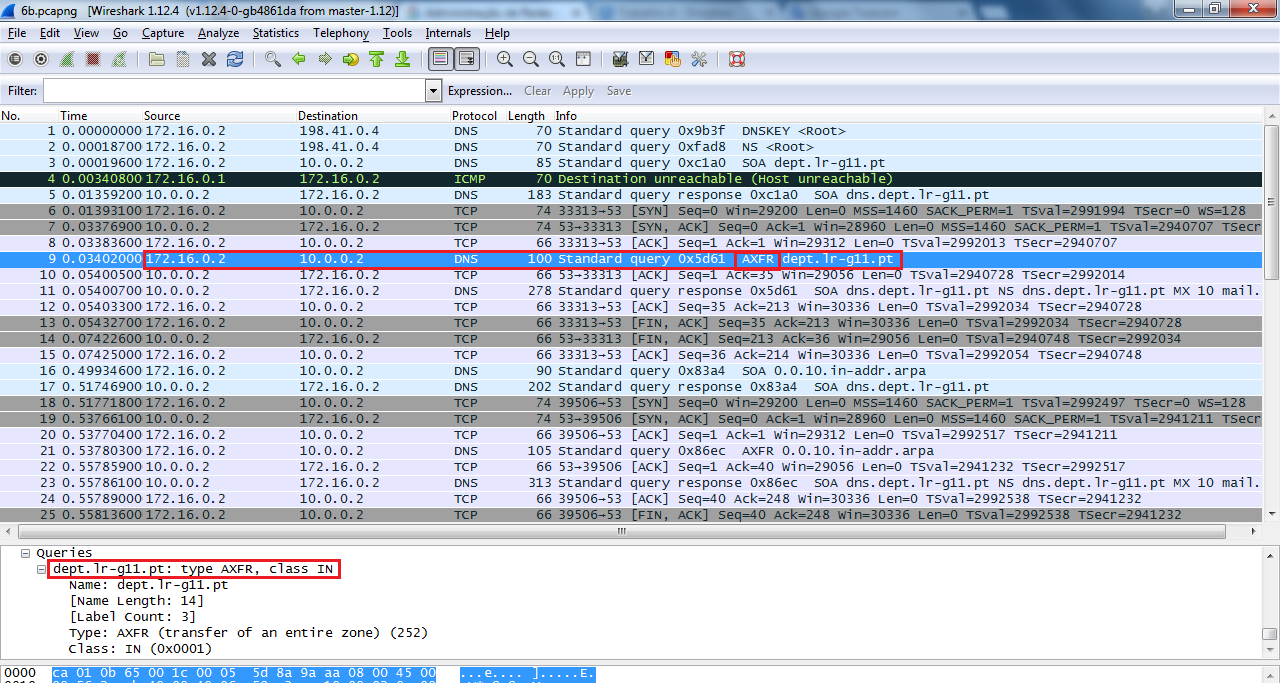
\includegraphics[width=1\textwidth, height=0.38\textheight]{6b_cap.png}
\label{fig:2-capturaWireshark}
\caption{Captura \emph{wireshark} no \textsf{dns.dept.lr-gX.pt}.}
\end{figure}


\subparagraph{c.}
Antes da transferência de domínio é feito um outro pedido para o registo SOA. Explique para que serve este registo e por que razão é pedido antes de fazer a transferência de domínio. (texRes)


\subparagraph{d.}
Verifica alguma diferença entre o protocolo de transporte usado para a transferência de domínio e o normalmente usado para as outras perguntas DNS? Qual a razão para essa diferença? (texRes)


\subparagraph{e.}
Captura de pacotes na pseudo-interface \textsf{any} no dns.lr-gX.pt:

\begin{figure}[h]
\centering
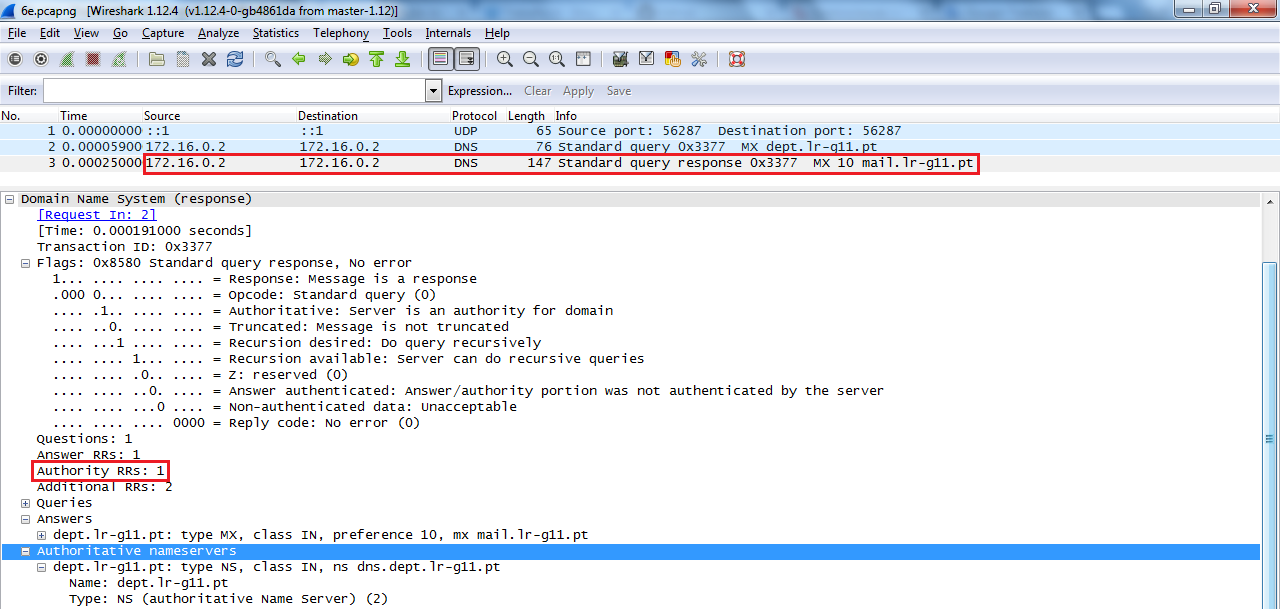
\includegraphics[width=0.85\textwidth, height=0.25\textheight]{6e_cap.png}
\label{fig:2-capturaWireshark}
\caption{Captura \emph{wireshark} no \textsf{dns.lr-gX.pt}.}
\end{figure}

\newpage
\subparagraph{f.}
A resposta que obteve na alínea anterior é autoritativa? Justifique. (texRes)


\paragraph{7.}

Conteúdo do ficheiro \textsf{named.ca}:

\begin{verbatim}
; <<>> DiG 9.9.2-P1-RedHat-9.9.2-6.P1.fc18 <<>> +bufsize=1200 +norec @a.root-servers.net
; (2 servers found)
;; global options: +cmd
;; Got answer:
;; ->>HEADER<<- opcode: QUERY, status: NOERROR, id: 25828
;; flags: qr aa; QUERY: 1, ANSWER: 13, AUTHORITY: 0, ADDITIONAL: 23

;; OPT PSEUDOSECTION:
; EDNS: version: 0, flags:; udp: 512
;; QUESTION SECTION:
;.				IN	NS

;; ANSWER SECTION:
.			518400	IN	NS	a.root-servers.net.
.			518400	IN	NS	b.root-servers.net.
.			518400	IN	NS	c.root-servers.net.
.			518400	IN	NS	d.root-servers.net.
.			518400	IN	NS	e.root-servers.net.
.			518400	IN	NS	f.root-servers.net.
.			518400	IN	NS	g.root-servers.net.
.			518400	IN	NS	h.root-servers.net.
.			518400	IN	NS	i.root-servers.net.
.			518400	IN	NS	j.root-servers.net.
.			518400	IN	NS	k.root-servers.net.
.			518400	IN	NS	l.root-servers.net.
.			518400	IN	NS	m.root-servers.net.

;; ADDITIONAL SECTION:
a.root-servers.net.	3600000	IN	A	198.41.0.4
a.root-servers.net.	3600000	IN	AAAA	2001:503:ba3e::2:30
b.root-servers.net.	3600000	IN	A	192.228.79.201
c.root-servers.net.	3600000	IN	A	192.33.4.12
d.root-servers.net.	3600000	IN	A	199.7.91.13
d.root-servers.net.	3600000	IN	AAAA	2001:500:2d::d
e.root-servers.net.	3600000	IN	A	192.203.230.10
f.root-servers.net.	3600000	IN	A	192.5.5.241
f.root-servers.net.	3600000	IN	AAAA	2001:500:2f::f
g.root-servers.net.	3600000	IN	A	192.112.36.4
h.root-servers.net.	3600000	IN	A	128.63.2.53
h.root-servers.net.	3600000	IN	AAAA	2001:500:1::803f:235
i.root-servers.net.	3600000	IN	A	192.36.148.17
i.root-servers.net.	3600000	IN	AAAA	2001:7fe::53
j.root-servers.net.	3600000	IN	A	192.58.128.30
j.root-servers.net.	3600000	IN	AAAA	2001:503:c27::2:30
k.root-servers.net.	3600000	IN	A	193.0.14.129
k.root-servers.net.	3600000	IN	AAAA	2001:7fd::1
l.root-servers.net.	3600000	IN	A	199.7.83.42
l.root-servers.net.	3600000	IN	AAAA	2001:500:3::42
m.root-servers.net.	3600000	IN	A	202.12.27.33
m.root-servers.net.	3600000	IN	AAAA	2001:dc3::35

;; Query time: 78 msec
;; SERVER: 198.41.0.4#53(198.41.0.4)
;; WHEN: Mon Jan 28 15:33:31 2013
;; MSG SIZE  rcvd: 699
\end{verbatim}

Observe o conteúdo desse ficheiro e explique a sua função. (texRes)